\section{Пружинка}
Рассмотрим уравнение пружины:
\begin{equation}
    F_{\text{elt}} = -kx, \quad F = ma
\end{equation}
Запишем уравнение пружины с внешним воздействием $F_{\text{ext}}$:
\begin{equation}
    m\ddot{x} = -kx + F_{\text{ext}}
\end{equation}
Запишем его в виде передаточной функции:
\begin{equation}
    W(s) = \frac{1}{ms^2 + k} = \frac{1/k}{T^2s^2 + 1}, \quad T = \sqrt{\frac{m}{k}}
\end{equation}
Получаем консервативное звено
\subsection{Временные характеристики}
\noindent Найдем весовую функцию системы:
\begin{equation}
    y_{\text{i.r.}}(t) = L^{-1}\left\{\frac{1}{k}\cdot\frac{1}{T^2s^2 + 1}\right\} = \frac{1}{kT}\sin\left(\frac{t}{T}\right)
\end{equation}
Найдем переходную функцию:
\begin{equation}
    y_{\text{s.r.}}(t) = L^{-1}\left\{\frac{1}{k}\cdot\frac{1}{T^2s^2 + 1}\cdot\frac{1}{s}\right\} = \frac{1}{k} \left(1 - \cos\left(\frac{t}{T}\right)\right)
\end{equation}

Сравнительные графики весовой и переходной функций, полученных аналитически и в ходе эксперимента  приведены на рис. \ref{fig:task4_impulse_response_cmp} и рис. \ref{fig:task4_step_response_cmp}.
\begin{figure}[ht!]
    \centering
    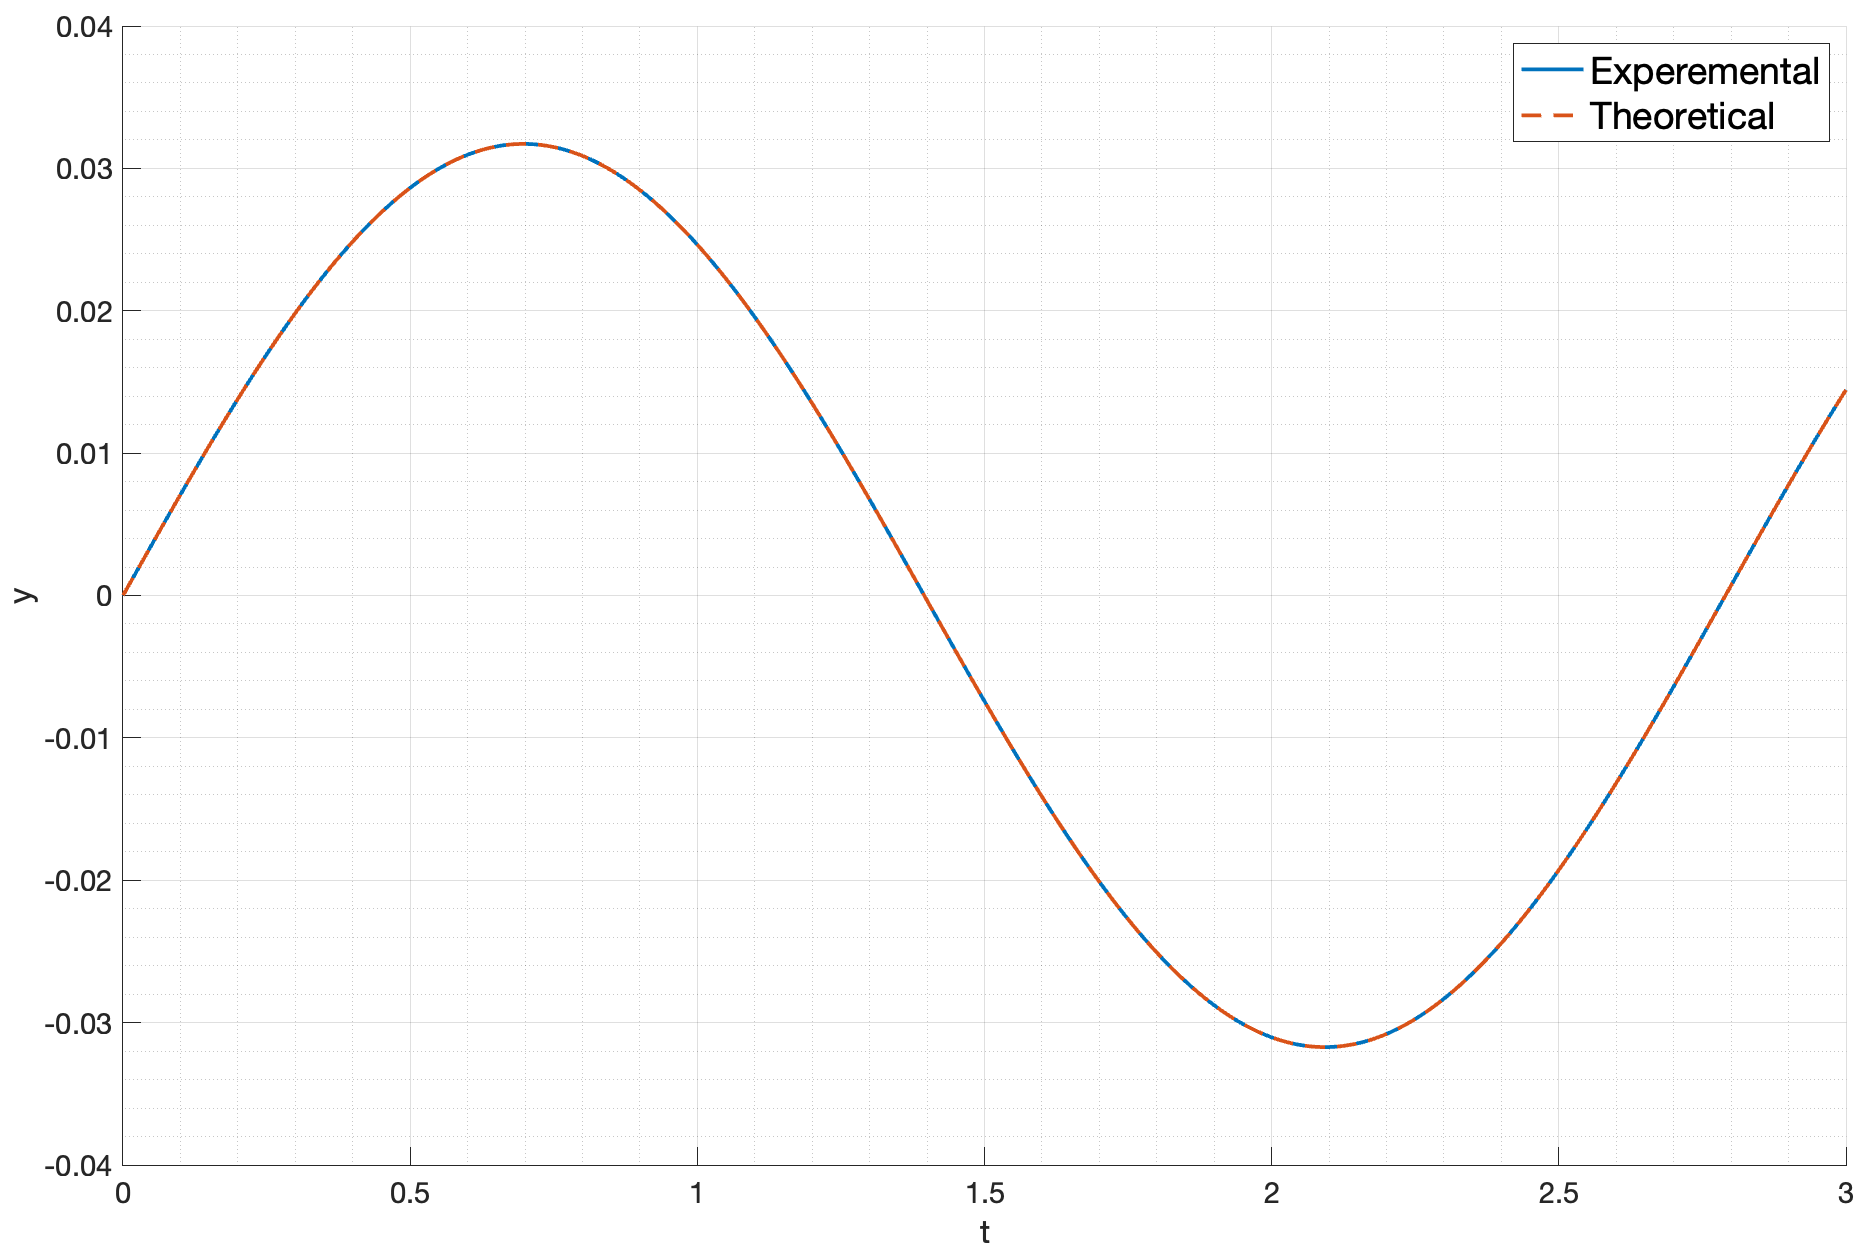
\includegraphics[width=\textwidth]{media/plots/task4_impulse_response_cmp.png}
    \caption{Сравнение весовых функций пружины}
    \label{fig:task4_impulse_response_cmp}
\end{figure}
\begin{figure}[ht!]
    \centering
    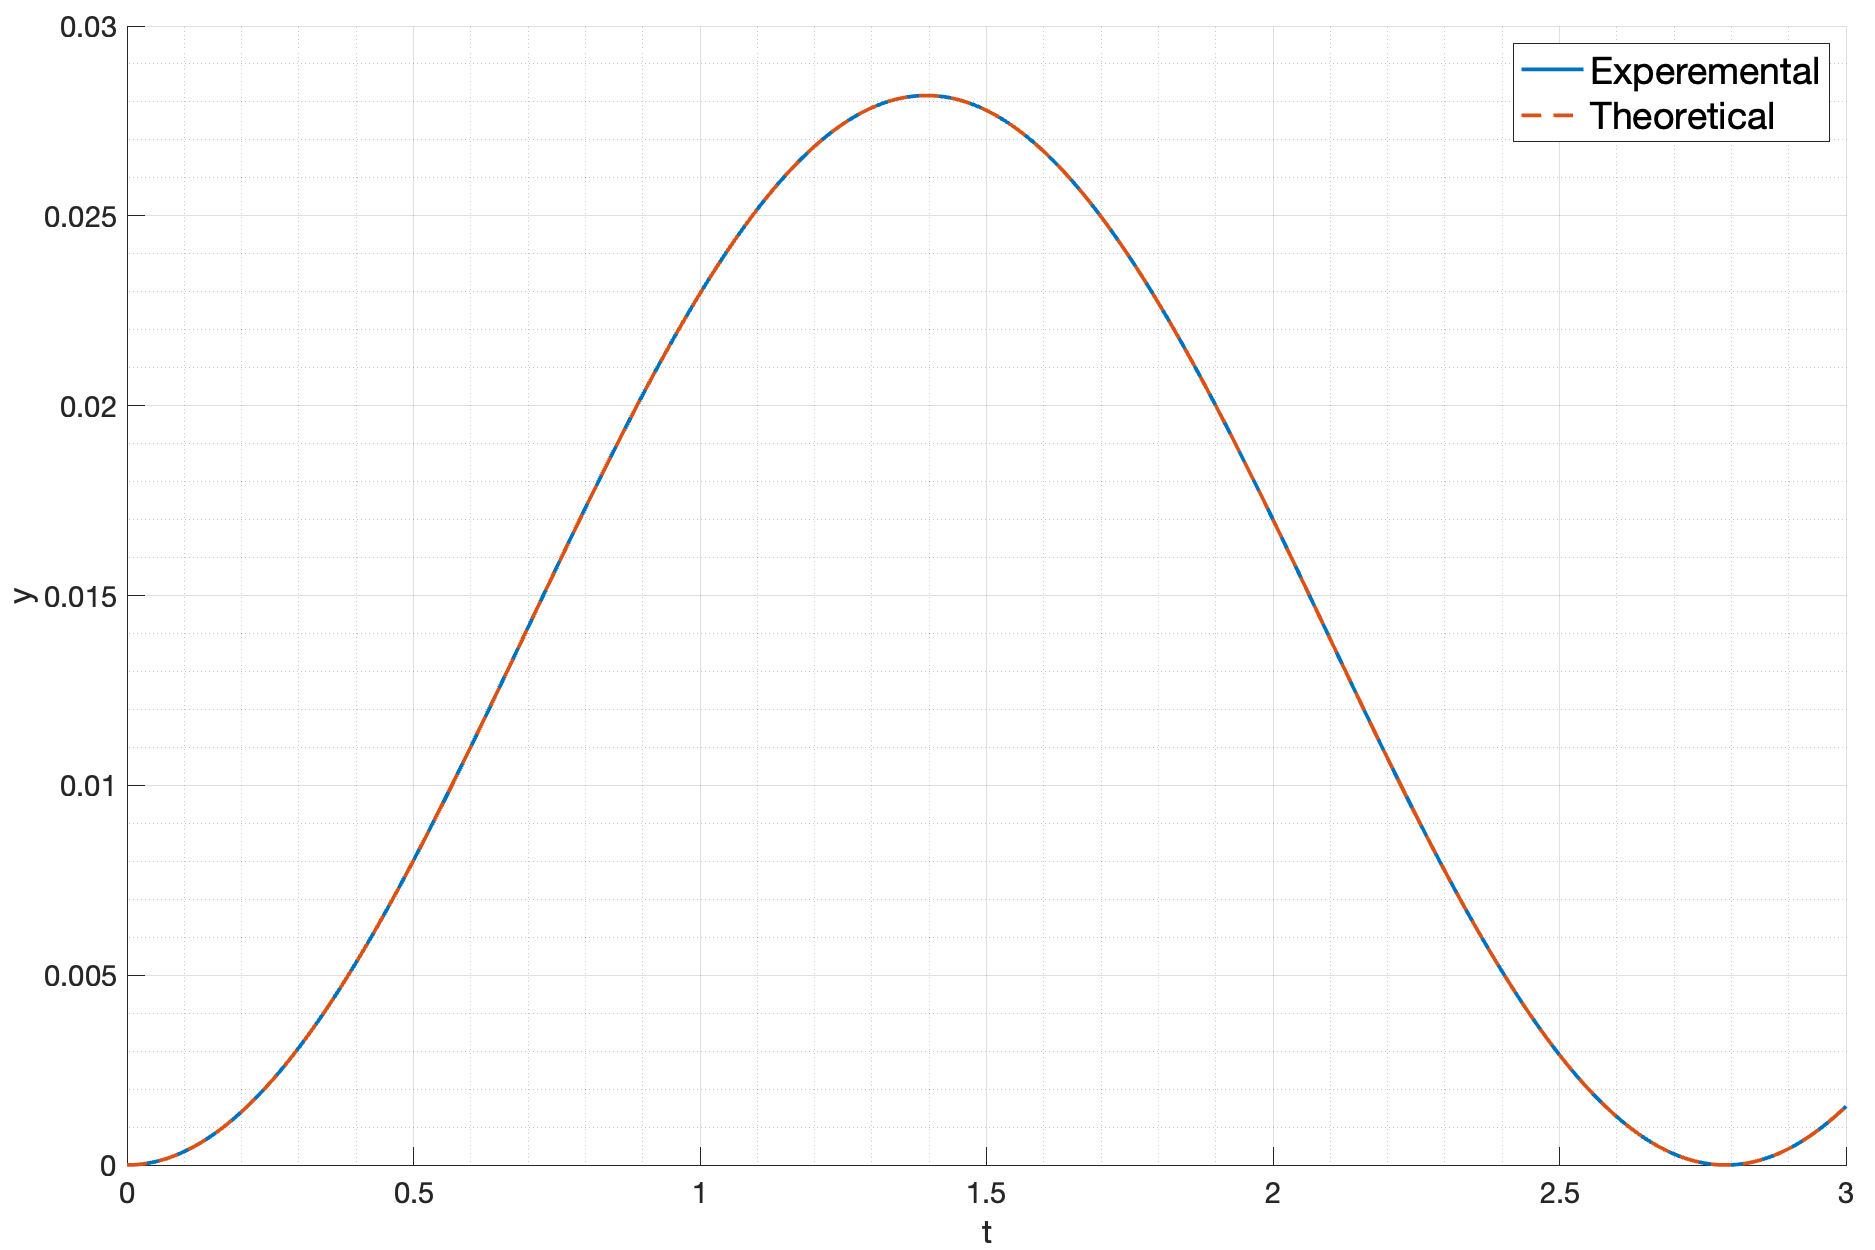
\includegraphics[width=\textwidth]{media/plots/task4_step_response_cmp.png}
    \caption{Сравнение переходных функций пружины}
    \label{fig:task4_step_response_cmp}
\end{figure}

\FloatBarrier
\subsection{Частотные характеристики}
\noindent Найдем амплитудно-частотную характеристику и фазо-частотную характеристику,
\begin{equation}
    W(j\omega) = \frac{1/k}{T^2(j\omega)^2 + 1} = \frac{1/k}{1 - T^2\omega^2}
\end{equation}
Найдем АЧХ:
\begin{equation}
    A(\omega) = \frac{1/k}{|1 - T^2\omega^2|}
\end{equation}
ФЧХ:
\begin{equation}
    \varphi(\omega) = -\text{atan2}\left(0,~1 - T^2\omega^2\right)
\end{equation}
Найдем логарифмическую АЧХ: 
\begin{equation}
    L(\omega) = 20\lg(A) = -20\lg(k) - 20\lg(|1 - T^2\omega^2|)
\end{equation}

Сравнительные графики АЧХ, ФЧХ, ЛАЧХ, полученных аналитически и в ходе эксперимента, приведены на рис. \ref{fig:task4_freq_resp_cmp_lin} и рис. \ref{fig:task4_freq_resp_cmp_loglog}.
\begin{figure}[ht!]
    \centering
    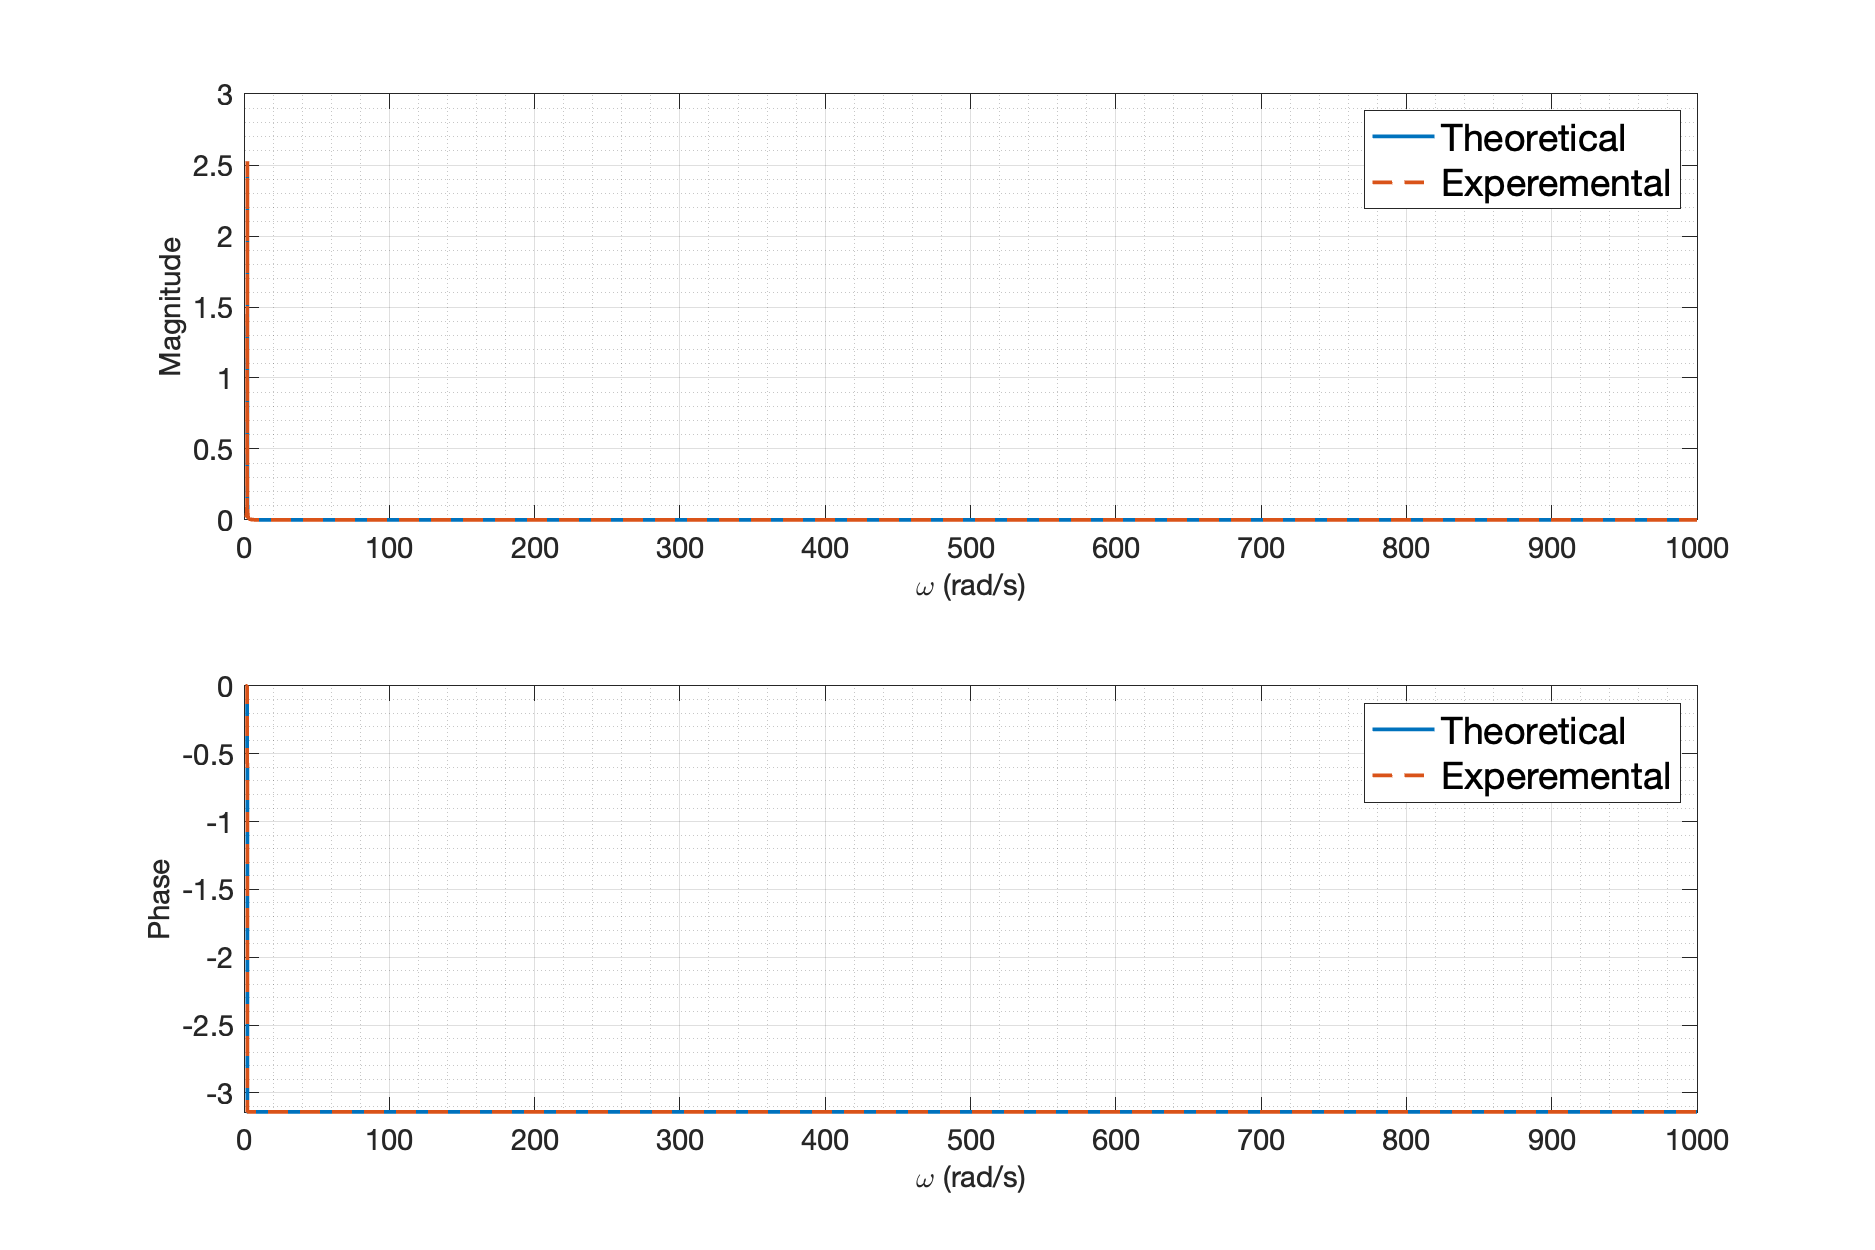
\includegraphics[width=\textwidth]{media/plots/task4_freq_resp_cmp_lin.png}
    \caption{Сравнение АЧХ и ФЧХ пружины}
    \label{fig:task4_freq_resp_cmp_lin}
\end{figure}
\begin{figure}[ht!]
    \centering
    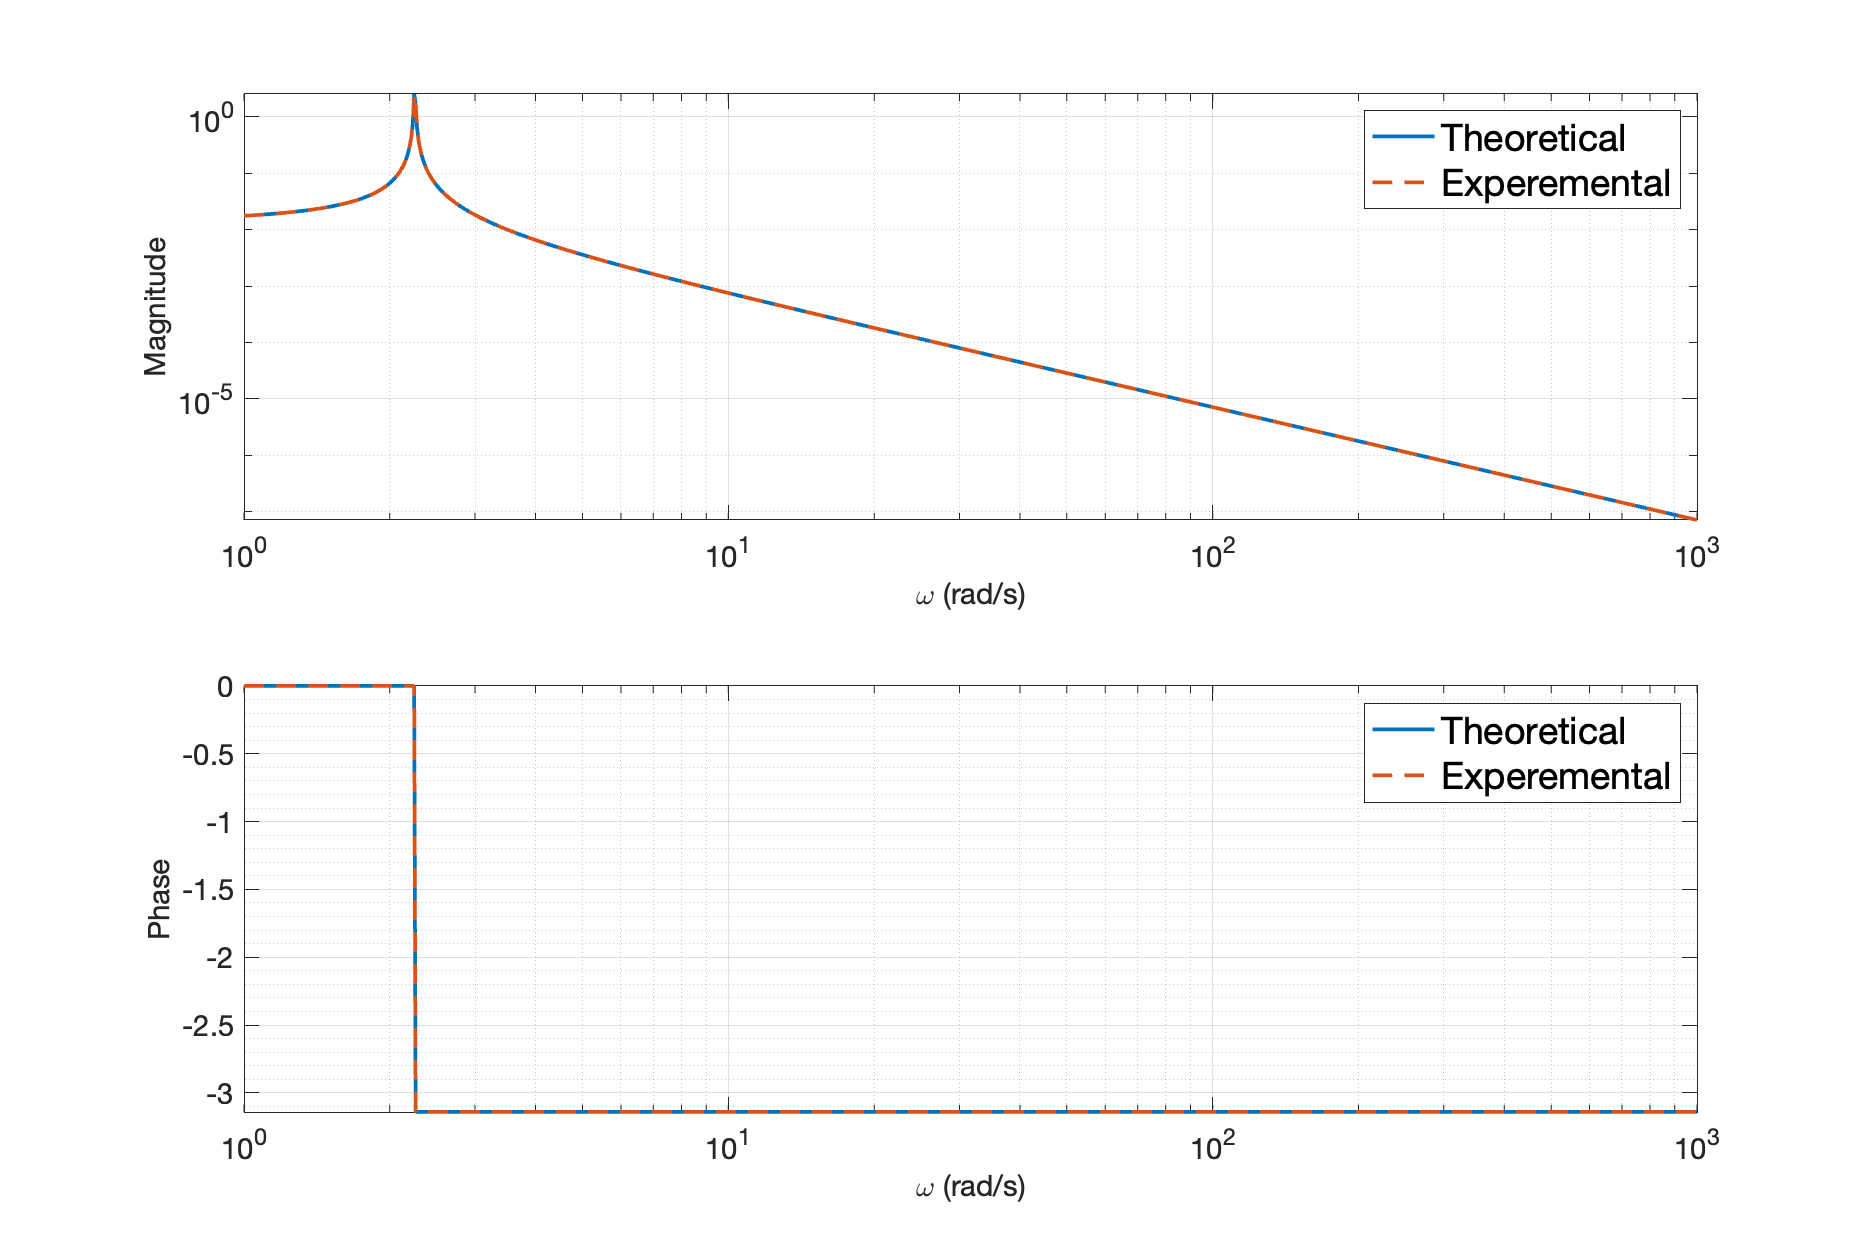
\includegraphics[width=\textwidth]{media/plots/task4_freq_resp_cmp_loglog.png}
    \caption{Сравнение логарифмической АЧХ пружины}
    \label{fig:task4_freq_resp_cmp_loglog}
\end{figure}